\documentclass[a4paper]{article}
\usepackage[utf8]{inputenc}
\usepackage[spanish]{babel} 
\renewcommand{\spanishtablename}{Tabla} 
\spanishdecimal{.}
\usepackage{verbatim}
\usepackage{amssymb}
\usepackage{subcaption}
\usepackage{wrapfig}
\usepackage{graphicx}
\usepackage{hyperref}
\usepackage{mathtools}
\usepackage{float}
\usepackage{siunitx}
\renewcommand{\thefootnote}{\arabic{fotnote}}
\setlength{\parskip}{\baselineskip} 
\usepackage{pdfpages}

\begin{document}

\begin{titlepage}
\paragraph{}

\begin{center}
\vspace*{0.10in}
\begin{figure}
\raggedleft

\includegraphics[scale=0.12]{unam.png}
\hspace{7.2cm}
\raggedright
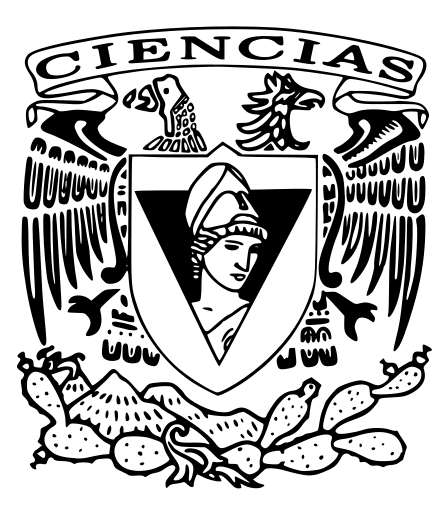
\includegraphics[scale=0.15]{fac.png}    
\end{figure}
\vspace*{0.5in}
UNIVERSIDAD NACIONAL AUTÓNOMA DE MÉXICO\\
\vspace*{0.2in}
FACULTAD DE CIENCIAS \\
\vspace*{0.5in}
\begin{large}
Laboratorio de Calor, Ondas y Fluidos\\
\end{large}
\vspace*{0.2in}
\begin{Large}
\textbf{Práctica 9} \\
\textbf{Viscosidad} \\
\end{Large}
\vspace*{0.3in}
\vspace*{0.3in}
\rule{80mm}{0.1mm}\\
\vspace*{0.1in}
\begin{large}
Profesor:  Quintanar Robles, Luis  \\
Ayudante: Quintanar Cortés, Luis Enrique \\
Mesa 1\\
Fecha de la práctica: 27 de agosto de 2019.\\
Alumnos: León Arenal Sebastian.\\
Robledo Ibarra Emiliano. \\
Toledo Castañeda Akim Tarik.\\
Velázquez Cebada Hannia Alexia.\\

\end{large}
\end{center}
\end{titlepage}



\section*{Resumen.}
Se midió la viscosidad de tres fluidos. Se aprovechó que la viscosidad se puede manejar como una fuerza de fricción. Se obtuvieron, experimentalmente los valores: $(1.27\pm0.03) Ns/m^2$, $(8.2\pm0.5) Ns/m^2$ y $(0.27\pm0.02) Ns/m^2$; para la glicerina, shampoo y agua respectivamente. Se encontró una diferencia de dos décimas entre los valores experimentales y los valores teóricos esperados; lo cual sugiere una revisión el diseño experimental en cuanto a las condiciones de temperatura y las características del cuerpo utilizado para hacer las mediciones.


\section*{Introducción.}
El objetivo de ésta práctica es encontrar la velocidad límite con la que caen pelotas de diferentes masas en distintos fluidos (glicerina, shampoo y agua) y verificar que existe una relación entre la velocidad con la que caen y la viscosidad del fluido.
Con frecuencia en la vida cotidiana se vierten fluidos en distintas ocasiones y es fácil notar que unos "fluyen" mejor que otros, esto se debe a una propiedad intrínseca a cada fluido llamada \textit{viscosidad}. Esta propiedad de los fluidos es "análoga" a la fricción en mecánica, pues se comporta de manera similar, oponiéndose al movimiento de la forma: $F_{r}=6\pi r \eta v_0$, siendo $\eta$ la viscosidad. Con esta "fricción" se puede hacer el análisis de fuerzas para las pelotas y el líquido en uso, quedando:

\begin{equation}
    \eta = \frac{2(\rho_o - \rho_l)gr^2}{9v_0}
\end{equation}
En la fórmula, $\rho_o$ es la densidad del pelota y $\rho_l$ la densidad del líquido, vemos que la fórmula cuenta con $v_0$ que se refiere a una velocidad después de un tiempo infinito, es por eso que se ajusta a las posibilidades del experimento donde es necesario encontrar la velocidad límite $v_L$:
\begin{equation}
    v_L = v_0 \left(1+2.4\frac{r}{R}\right)
\end{equation}
Donde $v_0$ representa la velocidad final (en un envase infinito), $v_L$ es la velocidad límite, $r$ es el radio del pelota y $R$ el radio del contenedor.

Para poder trabajar los datos son necesarias varias hipótesis. Las principales son acerca del fluido puesto que es el medio en el que se trabaja. Para relaciones hidrodinámicas se simplifican los fenómenos a no turbulentos, por lo cual se hará un análisis despreciando dicho comportamiento. Se consideró la densidad del fluido constante y su temperatura igual a la ambiente. Para la velocidad se observó sólo un eje (el vertical) puesto que se idealizó para que sólo hubiera cambios unidireccionales. Por último, se pensó en un objeto regular (esfera), para la pelota y se supuso densidad uniforme para la misma. 

\section*{Procedimiento.}

Se llenaron tres probetas grandes, una con agua, una con glicerina y una con shampoo. Se midió la altura de la columna de líquido dentro de cada probeta ($h$) con un flexómetro. Se midió el diámetro de cada probeta ($d_{R}$) con un vernier.

Se trabajó con tres pelotas de ping pong (una para cada fluido). Se calculó la masa de cada pelota ($m$) con una báscula; se midió el diámetro de cada pelota ($d_{r}$) con un vernier. Se calculó el volumen de cada pelota ($V$) y luego la densidad de cada una ($\rho$).

Para cada líquido se hizo el siguiente procedimiento:

1)Se colocó una cámara de 60 60 cps frente a la probeta de modo que la cámara registrara toda la probeta (como se muestra en la figura 1).

2)Se colocó una pelota de ping pong al ras de la superficie de cada fluido. Se dejó caer la pelota a través del fluido y se grabó la trayectoria con la cámara.

\begin{figure}[H]
    \centering
    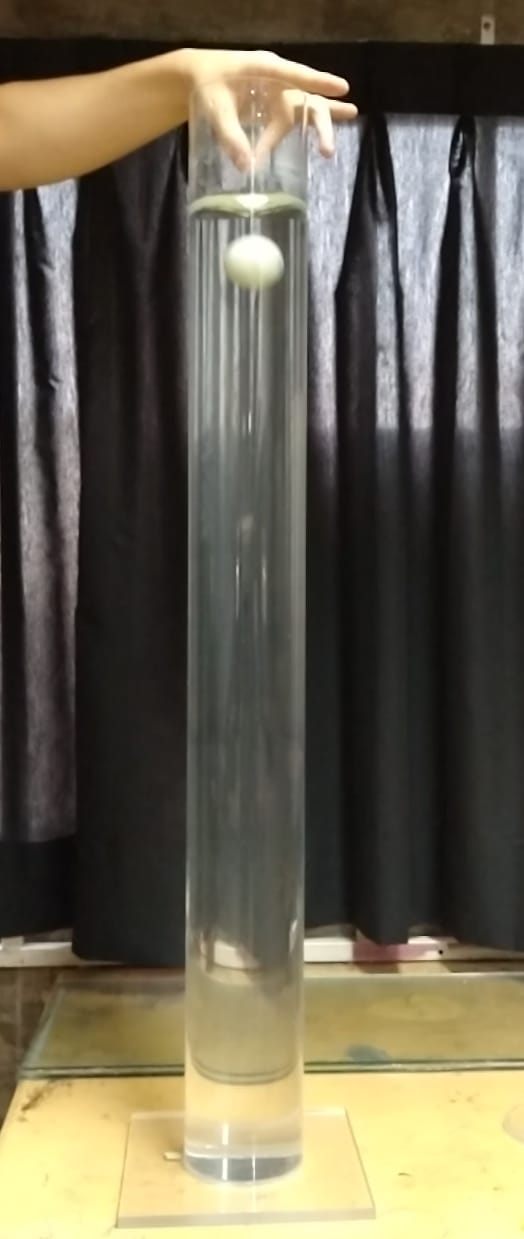
\includegraphics[width=8cm]{Viscosidadsistema.jpg}
    \caption{Se muestra el primer cuadro de un video del sistema con agua. Se observa claramente la totalidad de la probeta}
\end{figure}


3)Con ayuda de un gancho, se sacó la pelota del fondo de la probeta y se repitió el paso 2) diez veces para cada fluido. 

4)Utilizando las herramientas de trayectoria automática del programa Tracker, se obtuvieron datos de posición (en el eje perpedicular a la base de la probeta) y tiempo (considerando un intervalo desde que la pelota está completamente sumergida y hasta que toca por primera vez la base de la probeta) para cada una de las diez repeticiones de cada probeta. En total se registraron 30 tablas de datos de posición y tiempo.

5)Procesando los datos, se obtuvo una velocidad promedio (obtenida de los ajustes hechos con rectas a los datos de distancia contra tiempo con velocidad constante i.e. un ajuste lineal) y, a partir de ésta, se calculó un coeficiente de viscosidad para cada líquido utilizando las ecuaciones (1) y (2).

A todos los instrumentos de medición se les asignó una incertidumbre de la mitad de su mínima resolución. A los datos de longitud medidos con un vernier se les asignó una incertidumbre de $\pm0.002cm$. A los datos de longitud obtenidos con el flexómetro se les asignó $\pm0.05 cm$. A las masas medidas con la báscula se les asignó $\pm 0.05gr$ y a la velocidad se le otrogó la mayor de las incertidumbres obtenidas en los ajustes. Tanto al volumen de la esfera como a la viscosidad se le asignaron incertidumbres indirectas calculadas por su radio y por las variables con incertidumbre relacionadas al valor.



\section*{Resultados.}
Para esta sección se muestran los ajustes hechos a los datos obtenidos de posición contra tiempo de los videos analizados con Tracker. Se le ajustó una recta debido a que se esperaban velocidades constantes, esto son, funciones de la forma $y = mx+b$. Además se hace incapié en que la temperatura medida (ambiental) era de ($22.0\pm0.5$)ºC.

\subsubsection*{Glicerina}
Se reportan las medidas de los materiales utilizados para la medición de la viscosidad.
\begin{itemize}
    \item Diámetro del pelota: $d_r = (3.770\pm0.002)$ cm.
    \item Diámetro de la probeta: $d_R = (9.360\pm0.002)$ cm.
    \item Altura del líquido: $h = (67.00 \pm 0.05)$ cm.
    \item Masa del pelota: $m = (54.80\pm0.05)$ gr.
\end{itemize}
Y si obtenemos el volumen de la pelota se usó el de una esfera para después obtener la densidad:
\begin{equation}
    \rho_o = \frac{m}{V} = \frac{0.0548 kg}{2.8\times10^{-5} m^3} = (1953\pm8) kg/m^3
\end{equation}
Para obtener las velocidades se graficó y ajustó una recta (velocidad constante $mx+b$):
\begin{figure}[H]
    \centering
    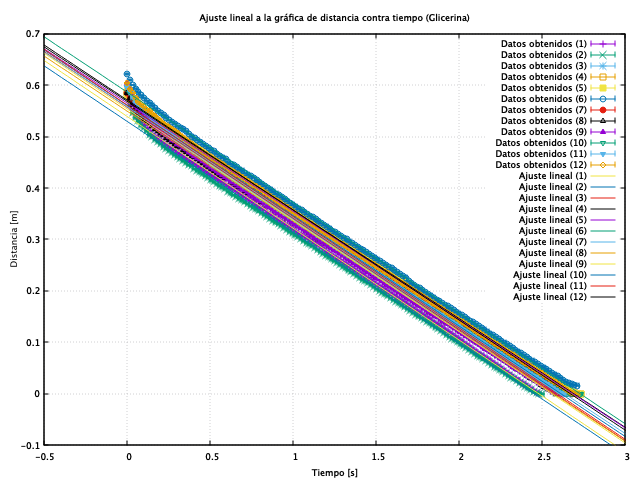
\includegraphics[width=10cm]{Glicerina.png}
    \caption{Trayectorias de la glicerina con el ajuste a una recta de su velocidad.}
\end{figure}
Donde la pendiente promedio fue:
\begin{itemize}
    \item Glicerina: $ m_G = v_y = (-0.2145\pm0.0007) m/s$.
\end{itemize}
Y la velocidad límite es:
\begin{equation}
    v_0 = 0.2145 \left(1+ 2.4\frac{0.0377}{0.0936} \right) = (0.4218\pm0.0014) m/s
\end{equation}

Y por último el coeficiente de viscosidad es:

\begin{equation}
    \eta_G = \frac{2(1953-1260)(9.78)(0.0188)^2}{9(0.4218)} = (1.27 \pm 0.04) \frac{N}{m^2}s
\end{equation}

\subsubsection*{Shampoo}
Se reportan las medidas de los materiales utilizados para la medición de la viscosidad.
\begin{itemize}
    \item Diámetro del pelota: $d_r = (3.950\pm0.002)$ cm.
    \item Diámetro de la probeta: $d_R = (9.455\pm0.002)$ cm.
    \item Altura del líquido: $h = (68.00 \pm 0.05)$ cm.
    \item Masa de la pelota: $m = (48.30\pm0.05)$ gr.
\end{itemize}
\begin{equation}
    \rho_o = \frac{m}{V} = \frac{0.0483 kg}{3.2\times10^{-5} m^3} = (1497\pm6) kg/m^3
\end{equation}
Para obtener las velocidades se graficó y ajustó una recta (velocidad constante $mx+b$):
\begin{figure}[H]
    \centering
    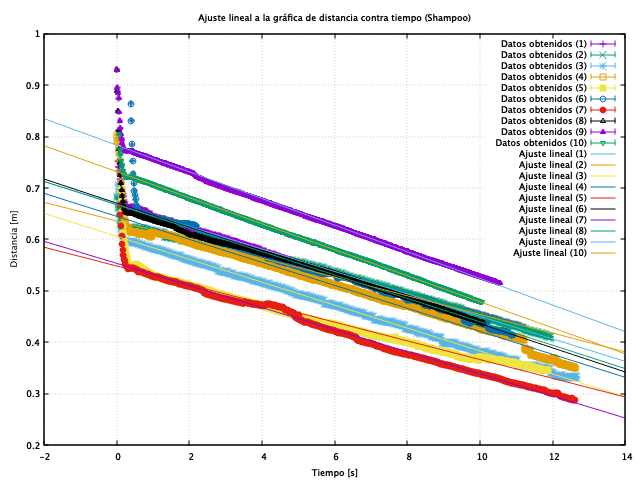
\includegraphics[width=10cm]{shampoo.png}
    \caption{Trayectorias del shampoo con el ajuste a una recta de su velocidad.}
\end{figure}
Y la pendiente promedio fue de:
\begin{itemize}
    \item Shampoo: $ m_S = v_y = (-0.0222\pm0.0003) m/s$.
\end{itemize}
Y la velocidad límite es:
\begin{equation}
    v_0 = -0.0222 \left(1+ 2.4\frac{0.0395}{0.09455} \right) = (-0.0444\pm0.0014) m/s
\end{equation}

Y por último el coeficiente de viscosidad es:

\begin{equation}
    \eta_S = \frac{2(1497-1030)(9.78)(0.0188)^2}{9(0.0444)} = (8.2\pm0.5) \frac{N}{m^2}s
\end{equation}


\subsubsection*{Agua}
Se reportan las medidas de los materiales utilizados para la medición de la viscosidad.
\begin{itemize}
    \item Diámetro del pelota: $d_r = (3.930\pm0.002)$ cm.
    \item Diámetro de la probeta: $d_R = (9.460\pm0.002)$ cm.
    \item Altura del líquido: $h = (89.00 \pm 0.05)$ cm.
    \item Masa del pelota: $m = (37.10\pm0.05)$ gr.
\end{itemize}

\begin{equation}
    \rho_o = \frac{m}{V} = \frac{0.0371 kg}{3.17\times10^{-5} m^3} = (1167\pm5) kg/m^3
\end{equation}

Para obtener las velocidades se graficó y ajustó una recta (velocidad constante $mx+b$):
\begin{figure}[H]
    \centering
    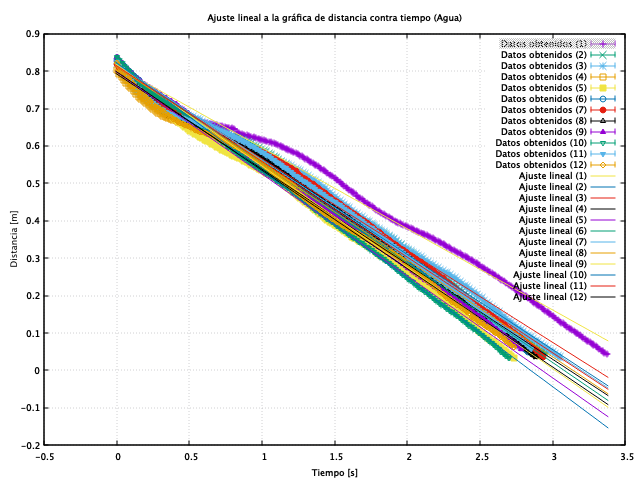
\includegraphics[width=10cm]{agua12.png}
    \caption{Trayectorias del agua con el ajuste a una recta de su velocidad.}
\end{figure}

Las pendiente promedio obtenida es:
\begin{itemize}
    \item Agua: $ m_A = v_y = (-0.2584\pm0.0017) m/s$
\end{itemize}
Y la velocidad límite es:
\begin{equation}
    v_0 = 0.2584 \left(1+ 2.4\frac{0.0393}{0.0946} \right) = (0.5160\pm0.0014) m/s
\end{equation}


Y por último el coeficiente de viscosidad es:

\begin{equation}
    \eta_A = \frac{2(1497-1030)(9.78)(0.0188)^2}{9(0.4218)} = (0.27\pm0.02) \frac{N}{m^2}s
\end{equation}


\section*{Conclusiones.}
Podemos ver los resultados numéricos finales de la glicerina, shampoo y el agua: $(1.27\pm0.03) Ns/m^2$, $(8.2\pm0.5) Ns/m^2$ y $(0.27\pm0.02) Ns/m^2$. Comparando el resultado de la viscosidad de la glicerina  obtenida con lo que reportan libros: 1.5$N/m^2s$) [1], observamos que se aleja dos décimas del obtenido en el experimento, lo cual hace notar que hay condiciones externas que no se tomaron en cuenta; sabemos que el objeto es irregular en cuanto a la distribución de su masa (puesto que contenía balines dentro) lo cual altera su densidad, suponer que contaba con una densidad regular i.e. una distribución de masas homogénea significa caer en un error y ,como podemos ver, la densidad del objeto desarrolla un papel fundamental en el cálculo. Además de esto es necesario aclarar que la viscosidad depende de la temperatura de cada fluido y ésta no fue medida porque se consideró constante e igual a 22 grados Celsius. 

En el caso del agua se tiene una viscosidad teórica de $0.001 Ns/m^2$. Pero para este líquido se observó un fenómeno adicional debido al paso de la pelota, la turbulencia. Lo que ocurría era que la pelota se movía de lado a lado y por esto variaba su paso a través de la misma. Es decir, su movimiento dentro del mismo fluido era algo aleatorio. Es así como además de la turbulencia, la densidad de la pelota (como se mencionó antes) afectaron a la obtención de la viscosidad en este caso. 

En el caso del shampoo, ya que no se cuenta con una ficha técnica del shampoo utilizado, sólo podemos darnos idea de los valores cercanos al resultado deseado; buscando un producto similar podemos ver que se encuentra muy cercano el valor que se encontró experimentalmente; un producto similar tiene un coeficiente de $7 Ns/m^2$ [3], el cual difiere en 1.2 unidades del experimentalmente obtenido, sin embargo este coeficiente (el de referencia) se midió a 30ºC lo cual hace que la referencia sea únicamente en la magnitud puesto que sabemos que la temperatura es un factor que altera la viscosidad de un fluido y de hecho ambos líquidos tienen densidades similiares lo cual nos puede decir que nuestro producto a 30ºC puede tener una viscosidad cercana a los $7 Ns/m^2$.

En general, los resultados obtenidos resultan ser lo suficientemente cercanos a los cuales se esperó obtener de tal forma que podemos ver que las variables se relacionan de la manera esperada, pero aún podemos dudar acerca de dicha relación ya que se encontraron hipótesis y fenómenos no considerados u omitidos que afectaron, en mayor o menor medida, al valor final. Aspectos como la turbulencia debida al paso del objeto en el fluido, la distribución de masas no fija e irregular, la imperfección entre objetos considerados regulares y las densidades no homogéneas o supuestas. Estos factores ignorados hacen que las mediciones puedan mejorarse cambiando los objetos y los recipientes para poder aseverar que en realidad la relación utilizada expresa la viscosidad y sobre todo, es una buena descripción.









\section*{Bibliografía}
\begin{thebibliography}{a}
\bibitem{pradery} \textsc{Sears, F., Zemansky, M., Young, H., Freedman, R.} (2009). \textit{Física universitaria volumen 1}. ($12^a$ ed). México. PEARSON EDUCACIÓN.

\bibitem{pradery} \textsc{Bevington P., Robinson D.} (1969). \textit{Data Reduction and Error Analysis for the Physical Sciences
}. ($3^a$ ed). México. Mc Graw Hill.


\bibitem{pradery} \textsc{Diversey España.} (2010). \textit{Soft Care Dove Shampoo.}. ($1^a$ed) [ebook]. Barcelona, p.1. Disponible en: http://diverseysolutions.com/ProductDocuments/eb814da2ec964aac87eeff99a979cfcb.pdf.

\bibitem{pradery} \textsc{Batchelor, G.K.} (1967). \textit{An Introduction to Fluid Dynamics}. Cambridge University 

\end{thebibliography}

\end{document}


